\section{Electrothermal Thrusters}

\subsection{Introduction}

Electrothermal propulsion comprises all techniques whereby a propellant gas is heated electrically and then expanded through a nozzle to convert its thermal energy to a jet of directed kinetic energy. In this chapter we shall consider two substantially different electrical means for heating the propellant flow:
\begin{enumerate}
    \item by passing it over an electrically heated solid surface, the so-called \textit{resistojet};
    \item by passing it through an arc discharge, usually termed an \textit{arcjet}.
\end{enumerate}
In each case we shall find that the attainable exhaust velocity is determined primarily by the maximum temperature that the chamber and nozzle surfaces can tolerate and by the gas-kinetic and thermodynamic properties of the propellant gas (\cite{pep_book} p. 90).

\subsection{Performances}

The gross performance of accelerators of this class can be forecast by reference to a general conceptual model. Electrical power from an external supply of given capacity $P$ is delivered in some manner to heat a propellant stream in a suitable chamber to some maximum temperature $T_c$. The electrically heated gas is then allowed to expand through a supersonic nozzle to a low pressure determined by the nozzle area ratio and by the chamber pressure $P_c$ (\cite{pep_book} p. 91).

Under the assumptions of one-dimensional adiabatic constant specific heat expansion through the nozzle, the attainable exhaust speed $u_e$ may be written from a simple energy balance \cite{pep_book} p. 91):
\begin{equation}
    \frac{1}{2} u_e^2 + C_p T_e = C_p T_{0c}
\end{equation}
By substituting the isentropic flow relations into the energy balance equation, we obtain the standard expression for the exit velocity:
\begin{equation}
    u_e = \sqrt{\frac{2\gamma}{\gamma-1} \frac{R_o T_c}{\mathcal{M}} \left[ 1 - \left( \frac{p_e}{p_c} \right)^{\frac{\gamma-1}{\gamma}} \right]}
\end{equation}

Assuming that the expansion is infinite where exit pressure is zero, the equation becomes:
\begin{equation}
    u_e = \sqrt{2 C_p T_c}
\end{equation}

The constant-pressure specific heat of the propellant gas per unit mass $C_p$ is seen to be a particularly critical quantity, since it defines the stagnation enthalpy which can be imparted to the gas at a given temperature, and thereby limits the attainable exhaust velocity (\cite{pep_book} p. 91).

Other parameters that characterize the performance of electrothermal thrusters are: thrust coefficient $C_F$, characteristic velocity $C^*$, specific impulse $I_{sp}$, and various efficiencies, as used in chemical rocket engines. The specific impulse $I_{sp}$ can be related to thrust coefficient $C_F$ and characteristic velocity $C^*$, as given in the following:
\begin{equation}
    I_{sp} = \frac{C_F C^*}{g_0}
\end{equation}

Note that the characteristic velocity $C^*$ does not depend on the method of heating of the propellant gas, which can be observed from the following expression:
\begin{equation}
    C^* = \sqrt{ \frac{1}{\gamma}{\frac{R_o T_c}{\mathcal{M}}}{\left( \frac{\gamma+1}{2} \right)^{\frac{\gamma+1}{\gamma-1}}} }
\end{equation}

In electrothermal rockets, the characteristic velocity $C^*$ depends only on the molecular weight, specific heat ratio, and temperature of propellant gas as in the case of chemical rocket (\cite{fund_rocket_prop} p. 407). 

Now that we have defined the characteristic velocity, we can say that the mass flow rate $\dot{m}$ through the nozzle can be as follows:
\begin{equation}
    \dot{m} = \frac{p_c A_t}{C^*}
\end{equation}
The relation for choked mass flux can be easily obtained by substituting Equation (5) in Equation (6) as follows:
\begin{equation}
    \dot{m} = \frac{p_c A_t}{\sqrt{T_c}}\sqrt{\frac{\gamma}{\frac{R_o}{\mathcal{M}}}\left(\frac{2}{\gamma+1}\right)^{\frac{\gamma+1}{\gamma-1}}}
\end{equation}

The last important equation is about the thrust $F$, that we can express as:
\begin{equation}
    F = \dot{m} u_e + (p_e - p_a) A_e
\end{equation}
where the first and second terms represent the momentum contribution and pressure components of thrust, respectively. The maximum thrust can be obtained only when the nozzle exhaust pressure is equal to the ambient pressure ($p_e = p_a$):
\begin{equation}
    F_{max} = \dot{m} u_e
\end{equation}

The nonideality of an electrothermal accelerator can be catalogued by defining the partial efficiency with which electric energy is delivered from the source to heat the gas stream, $\eta_h$; the aerodynamic, or nozzle, efficiency with which the stream follows a one-dimensional adiabatic route through the expansion process, $\eta_a$; and the efficiency with which it converts internal energy in the propellant stream to directed kinetic energy, $\eta_f$. 

As such, $1-\eta_h$ accounts for losses in the heating process; $1-\eta_a$ covers the nozzle viscous and profile losses; $1-\eta_f$ describes the unrecovered internal energy in the exhaust jet, often called frozen flow losses. It is essential that the overall thruster efficiency $\eta = \eta_h \eta_a \eta_f$ be kept high if the complete electrothermal propulsion system is to retain its advantage over chemical rockets (\cite{pep_book} p. 93).



\section{Resistojets}

\subsection{Principles}
The resistojet is the simplest of all electrical thrusters, consisting of an electrically heated pressure chamber and a convergent–divergent nozzle similar to the chemical rocket engine. In this case, the propellant gas is heated by making it come into contact with an electrically heated solid surface (\cite{fund_rocket_prop} p. 405).
Some of the heating elements for resistojets are shown in Figure 1.
\begin{figure}[H]
    \centering
    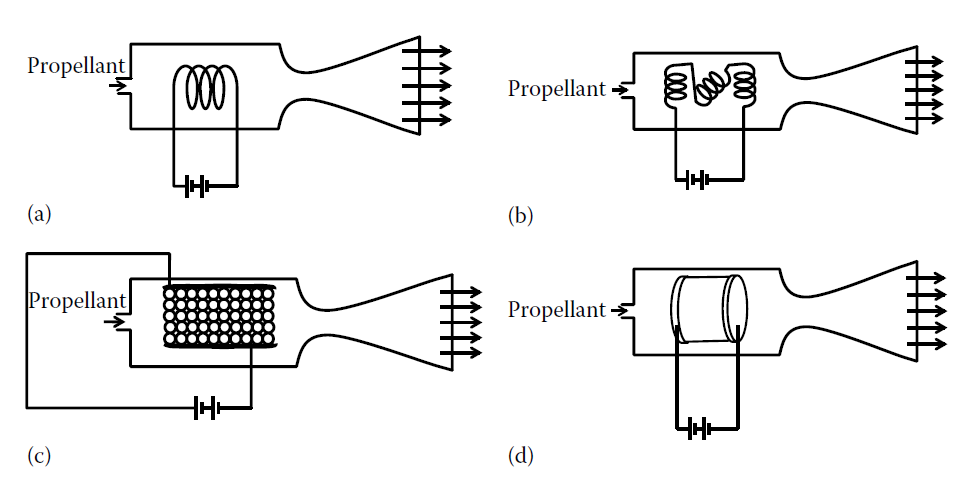
\includegraphics[width=0.5\linewidth]{figs/resistojet_pic1.png}
    \caption{Four types of electrical heating elements for resistojets: (a) straight coiled wire, (b) transverse coiled wire, (c) sphere bed, and (d) chamber wall.}
    \label{resistojet_schematics}
\end{figure}

In the case of straight coiled wire resistojet, propellant passes along the heating element, which restricts the heating rate of the propellant. In order to improve the heating rate of the propellant, heating coils can be placed in transverse direction of flow. A bed of tungsten spheres is used to heat the propellant by passing current through the contact resistances of spheres. However, it enhances the bulkiness while incurring significant pressure losses. 

The performance of such kind of resistojets depends on the extent of heat transfer from resistance element to the propellant gas stream and radiative heat transfer from the complete assembly as heat loss through the walls is basically a loss of power in the thruster (\cite{fund_rocket_prop} p. 406).

\subsection{Energy Balance}
The electrical energy is transformed into heat. This is defined as the Joule heating effect. The theoretical heat can be calculated using the following energy balance equation:
\begin{equation}
    P_{elec} = I^2 R = \dot{m} C_p (T_c - T_{in}) + \dot{Q}_{loss}
\end{equation}
For ideal heating, electrical energy equals heat energy (\cite{resjet} p. 165). We can define the heat transfer efficiency $\eta_h$, so we can rewrite the energy balance as:
\begin{equation}
    \eta_h P_{elec} = \dot{m} C_p (T_c - T_{in})
\end{equation}

A design objective in resistojets is to keep heat losses in the chamber low relative to the power consumed. This can be done by: (1) the use of external insulation; (2) internally located radiation shields; (3) entrant flow layers or cascades.
Another important reason for heat-isolation is to keep any stored propellant from overheating under all operating conditions (\cite{Sutton2016-RPE9th} p. 633).

In the case of a chemical rocket, temperature of propellant gas is dependent on the propellant composition and not on its mass flow rate. In contrast, in the electrothermal rocket, temperature is dependent inversely on the mass flow rate:
\begin{equation}
    T_c \propto \frac{P_{elec}}{\dot{m}}
\end{equation}

For a fixed power, if the mass flow rate is too small for a particular heat input, then the temperature may rise to spoil the heating element itself. Hence, an electrothermal thruster has a maximum flow rate/power ratio that is limited by the materials of filaments and chamber wall (\cite{fund_rocket_prop} p. 407).

Electrical energy can be lost due to (1) wasted electrical power (stray currents, ohmic resistances, etc.), (2) heat losses, (3) nonaxial component of exhaust, and (4) nonuniform heating of propellant (\cite{fund_rocket_prop} p. 408). 

The thruster efficiency $\eta$ can be defined as the ratio of the kinetic energy rate producing the thrust of the exhaust nozzle to the total electrical power, given as follows:
\begin{equation}
    \eta = \frac{\dot{m}u_e^2}{VI} = \frac{FI_{sp}g_o}{2VI}
\end{equation}
where $V$ is the voltage and $I$ is the current. Generally, the thruster efficiency of resistojets varies from 65\% to 90\% (\cite{fund_rocket_prop} p. 408).

\subsection{Specific Characteristics}
The highest specific impulse has been achieved with hydrogen (because of its lowest molecular mass), but its low density makes propellant storage too bulky (cryogenic storage is unrealistic for most space missions). Since virtually any propellant is appropriate, a large variety of different gases have been used,  such as $H_2O$, $CO_2$, $NH_3$, $CH_4$ and $N_2$ (\cite{Sutton2016-RPE9th} p. 633).

The major engineering problems of designing and developing resistojets is the fabricating and maintaining of the conducts and insulators that can keep electrical integrity and vacuum seals at high temperature in the range of 2500–3000 K (Mishra, 2017, p. 408). Resistojets are fundamentally temperature-limited by the available structural materials, which at present constrain them to a range of exhaust velocities below $10^{-4} \text{ m/s}$ and a maximum possible specific impulse of about 300 sec for typical storable propellants; however, resistojets that use hydrogen can go beyond 800 sec
(\cite{pep_book} p. 110).
 
Resistojet thrusters typically produce low thrust levels (10--200 mN, up to 1 N) with mass flow rates between $10^{-6}$ and $10^{-4}$ kg/s.
In spite of low values of thrust and mass flow rate, these thrusters are preferred for space applications. They are deployed for auxiliary but important applications during satellite operation, station keeping, drag neutralization, attitude control, and so on, where compactness, high reliability, and low thrust are called for (\cite{fund_rocket_prop} p. 409).